\documentclass[10pt, a4paper]{article}

% Packages
%======================================
% Page Geometry
\usepackage{geometry}
\geometry{a4paper, left=1in, right=1in, top=1in, bottom=1in, headheight=13.6pt}
%======================================
% Document spacing
% Line spacing
\usepackage{setspace}
\setstretch{1.2}
% Paragraph spacing
\usepackage[skip=2.5pt, indent=12pt]{parskip}
%======================================
% Headers and footnotes
\usepackage{fancyhdr}
%======================================
% Math packages
\usepackage{tikz}
% Norm command
\usepackage{physics}
\usepackage{tikz-cd}
\usepackage{mathtools}
\usepackage{amsmath,amssymb}
% Inline fractions
\usepackage{nicefrac}
% Overbar that fits
\newcommand{\overbar}[1]{\mkern 1.5mu\overline{\mkern-1.5mu#1\mkern-1.5mu}\mkern 1.5mu}
% Quotient space
\newcommand{\bigslant}[2]{{\raisebox{.2em}{$#1$}\left/\raisebox{-.2em}{$#2$}\right.}}
% Array stretch for matrices
\makeatletter
\renewcommand*\env@matrix[1][\arraystretch]{%
  \edef\arraystretch{#1}%
  \hskip -\arraycolsep
  \let\@ifnextchar\new@ifnextchar
  \array{*\c@MaxMatrixCols c}}
\makeatother
%======================================
% Theorem environments
\usepackage{amsthm}
\newtheoremstyle{BoldTopBottomSpacing}
  {0.7em} % Space above
  {0.7em} % Space below
  {} % Body font
  {} % Indent amount
  {\bfseries} % Head font
  {.} % Punctuation after head
  {0.5em} % Space after head
  {} % Head spec
\newtheoremstyle{BoldTopSpacing}
  {0.7em}
  {\topsep}
  {\itshape}
  {}
  {\bfseries}
  {.}
  {0.5em}
  {}
% Thereom
\theoremstyle{BoldTopSpacing}
\newtheorem{theorem}{Theorem}[section]
% Lemma
\theoremstyle{BoldTopSpacing}
\newtheorem{lemma}[theorem]{Lemma}
% Corollary
\theoremstyle{BoldTopSpacing}
\newtheorem{corollary}{Corollary}[theorem]
% Definition
\theoremstyle{BoldTopBottomSpacing}
\newtheorem{definition}{Definition}[section]
% Proposition
\theoremstyle{BoldTopSpacing}
\newtheorem{proposition}{Proposition}[section]
% Example
\theoremstyle{BoldTopBottomSpacing}
\newtheorem{example}{Example}[section]
% Remark
\theoremstyle{remark}
\newtheorem{remark}{\textit{Remark}}[section]
% Sketch of proof
\newenvironment{proofsketch}{%
  \renewcommand{\proofname}{Proof sketch}\proof}{\endproof}
%======================================
% German ß ä ö ü
\usepackage{lmodern}
\usepackage[T1]{fontenc}
\usepackage[main=english,german]{babel}
%======================================
% Quotation marks
\usepackage{csquotes}
%======================================
% Lists
\usepackage{enumitem}
%======================================
% Color
\usepackage{xcolor}
\definecolor{TUColor}{cmyk}{0, 1.0, 0.99, 0.40} % TU Dark Red
\definecolor{CitationColor}{cmyk}{0.9, 0.6, 0.0, 0.6} % Dark Blue
\definecolor{RichBlack}{cmyk}{0.75, 0.68, 0.67, 0.9}
%======================================
% Hyper links and references
\usepackage{hyperref}
\hypersetup{
    colorlinks,
    urlcolor={CitationColor},
    citecolor={CitationColor},
    linkcolor={RichBlack}
}
%======================================
% Citations
\usepackage[nobreak]{cite}
%======================================
% Images
\usepackage{float}
\usepackage{graphicx}
\graphicspath{{./images/}}
% Captions
\usepackage{subcaption}
\renewcommand\thesubfigure{\roman{subfigure}}
%======================================
% For Title page
\usepackage{tabularx, booktabs}
%======================================
% Fancy boxes
\usepackage[most]{tcolorbox}
\tcbuselibrary{skins,breakable}
\newtcolorbox{mathbox}[2][]{breakable, sharp corners, boxrule=0mm, leftrule=2mm, boxsep=0mm, arc=0mm, outer arc=0mm, opacityframe=0}
%======================================


\begin{document}
%===========================================================
% General settings
% Font color
\color{RichBlack}
% Redefine header "fancy" style
\fancypagestyle{fancy}{
    \fancyhead{}
    \fancyfoot{}
    \fancyhead[LE,RO]{\footnotesize\itshape\nouppercase{\rightmark}}
    \fancyhead[LO,RE]{\footnotesize\itshape\nouppercase{\leftmark}}
    \fancyfoot[C]{\footnotesize\itshape\nouppercase\thepage}
    \renewcommand{\headrulewidth}{0.4pt}
    \renewcommand{\footrulewidth}{0.0pt}
}
\fancypagestyle{tocstyle}{
  \fancyhead{}
  \fancyfoot{}
  \renewcommand{\headrulewidth}{0.4pt}
  \renewcommand{\footrulewidth}{0.0pt}
}
%===========================================================


% Title page
%===========================================================
\begin{titlepage}
% Defines a new command for horizontal lines, change thickness here
\newcommand{\HRule}{\rule{\linewidth}{0.5mm}}
\begin{center}


\includegraphics[width=0.15\textwidth]{TU-Berlin-Logo.png}\\[1cm]
\begin{otherlanguage}{german}
\textsc{\LARGE Technische Universit"at Berlin}\\[1.5cm]
\textsc{\large Fakult\"at 2}\\[0.5cm]
\textsc{\large Institut f\"ur Mathematik}\\[0.5cm]
\end{otherlanguage}

% Title
\setlength{\aboverulesep}{10pt}
\setlength{\belowrulesep}{13pt}
\begin{tabularx}{\textwidth}{ >{\centering\arraybackslash}X}
\midrule[0.5mm]
\huge\bfseries Circular cross sections of quadrics\\
\midrule[0.5mm]
\end{tabularx}

% Author and supervisor
\begin{minipage}{0.4\textwidth}
    \begin{flushleft}
        \large
        \textit{\textcolor{TUColor}{Author}}\\
        Sara \textsc{Samy}
    \end{flushleft}
\end{minipage}
~
\begin{minipage}{0.4\textwidth}
    \begin{flushright}
        \large
        \textit{\textcolor{TUColor}{Supervisor}}\\
        Dr. Jan \textsc{Techer}
    \end{flushright}
\end{minipage}

% Position the date 3/4 down the remaining page
\vspace{260 pt}
{\large\today}
\end{center}
\end{titlepage}
%===========================================================


%===========================================================
% Set Abstract page style to "fancy"
\pagestyle{fancy}
\section*{Abstract}
\label{sec:abstract}

\pagebreak
%===========================================================
% Set TOC page style to "tocstyle"
\pagestyle{tocstyle}
\renewcommand{\contentsname}{Contents}
\tableofcontents
\pagebreak
%===========================================================
\listoffigures
\pagebreak
%===========================================================
% Set all following pages style to "fancy"
\pagestyle{fancy}
\section{Introduction}
\label{sec:introduction}
\pagebreak
%===========================================================
\section{Circular sections of quadrics}
\label{sec:circular-sections-of-quadrics}

In this paper, the term \textit{quadric} stands for ellipsoids (including spheres), hyperboloids, and paraboloids. We do not consider singular surfaces of degree two like quadratic cones and cylinders or degenerate cases like planes or pairs of planes (Appendix \ref{appendix:quadrics}).

Before we start investigating circles on quadrics, we recall a few facts about the $n$-dimensional complex projective space, and introduce Euclidean geometry as a subgeometry of projective geometry in the next two subsections. \par

\subsection{The complex projective space $\mathbb{C}\mathbb{P}^n$}
\label{subsec:complex-projective-space}

A point in the complex projective space $\mathbb{C}\mathbb{P}^{n}$ is determined by $n + 1$ elements $(z_{0}, \dots, z_{n})$ of the field $\mathbb{C}$, not all simultaneously zero. Two $(n + 1)$-tuples $(z_{0}, \dots, z_{n})$ and $(z'_{0}, \dots, z'_{n})$ determine the same point if and only if there exists $\lambda \in \mathbb{C} \setminus \{ 0 \}$ such that $z_{i} = \lambda z_{i}'$ for $i = 0, \dots, n$. This defines an equivalence relation~$\sim$ on $\mathbb{C}^{n + 1} \setminus \{ 0 \}$, and we can identify the complex projective space $\mathbb{C}\mathbb{P}^n$ with the quotient space of $\mathbb{C}^{n + 1} \setminus \{ 0 \}$ under this equivalence relation:
\[
    \mathbb{C}\mathbb{P}^n \cong \bigslant{\left( \mathbb{C}^{n + 1} \setminus \{ 0 \} \right)}{\sim}.
\]
Any $(n+1)$-tuple defining a point $P$ is called a set of \textit{homogeneous coordinates} of $P$, and we write $P = [z_{0},\dots, z_{n}]$.\par

One way to express the equivalence relation on $\mathbb{C}^{n+1} \setminus \{ 0 \}$ is by stating that a linear subspace of dimension one in $\mathbb{C}^{n + 1}$ corresponds to a point in $\mathbb{C}\mathbb{P}^n$. Any $(k+1)$-dimensional linear subspace of $\mathbb{C}^{n + 1}$ can be similarly \enquote{projectivied} by associating to it a \textit{projective subspace} of $\mathbb{C}\mathbb{P}^n$ with projective dimension $k$.

\begin{definition}[]
\label{def:projective-subspace}
A $k$-dimensional projective subspace of $\mathbb{C}\mathbb{P}^n$ is a projective space $\mathbb{P}(U)$:
   \[
       \mathbb{P}(U) := \{ [z] \in \mathbb{C}\mathbb{P}^n : z \in U \}.
   \]
where $U$ is a $(k+1)$-dimensional linear subspace of $\mathbb{C}^{n+1}$.
\end{definition}

There are no arithmetic operations defined for points in a projective space, but we may use operations defined on linear subspaces to combine projective subspaces. \newline
If $\mathbb{P}(U_{1})$ and $\mathbb{P}(U_{2})$ are two projective subspaces, then their intersection or their \textit{meet }$ \mathbb{P}(U_{1}) \cap \mathbb{P}(U_{2})$ is the projective subspace $\mathbb{P}(U_{1} \cap U_{2})$, and we write
\[
\mathbb{P}(U_{1}) \wedge \mathbb{P}(U_{2}) := \mathbb{P}(U_{1} \cap U_{2}).
\]
Similarly, the projective span or the \textit{join} of $\mathbb{P}(U_{1})$ and $\mathbb{P}(U_{2})$ is the projective subspace $\mathbb{P}(U_{1} + U_{2})$, and we write
\[
\mathbb{P}(U_{1}) \vee \mathbb{P}(U_{2}) := \mathbb{P}(U_{1} + U_{2}).
\]

There is a natural embedding $\mathbb{C}^n \hookrightarrow \mathbb{C}\mathbb{P}^n$ which sends a point $(z_{0}, \dots, z_{n-1}) \in \mathbb{C}^n$ to its equivalent class $[z_{0},\dots, z_{n-1}, 1] \in \mathbb{C}\mathbb{P}^n$. This way we get all the \textit{affine points} of $\mathbb{C}\mathbb{P}^n$ with $z_{n} \neq 0$, since a point $[z_{0}, \dots, z_{n}]$ with $z_{n} \neq 0$ corresponds to the affine point $(z_{0}/z_{n}, \dots, z_{n-1}/z_{n}) \in \mathbb{C}^{n}$. The points of the complementary set with $z_{n} = 0$ are called \textit{points at infinity}. This notion depends on the choice of the coordinate $z_{n}$. In fact, $\mathbb{C}\mathbb{P}^n$ contains $n + 1$ isomorphic copies of the affine space $\mathbb{C}^n$:
\[
    U_{i} = \left\{ \left[ \frac{z_{0}}{z_{i}}, \dots, \frac{z_{n}}{z_{i}} \right] : z_{j} \in \mathbb{C} \ \text{for} \ j=0, \dots, n \ \text{and} \ z_{i} \neq 0 \right\} \cong \mathbb{C}^n, \quad \quad i=0, \dots, n.
\]
Every point in $\mathbb{C}\mathbb{P}^n$ is contained in at least one of these pieces, and can be written down in the affine coordinates of that piece [Figure~\ref{fig:affine-patches-diagram}].\par

\begin{figure}[H]
    \centering
    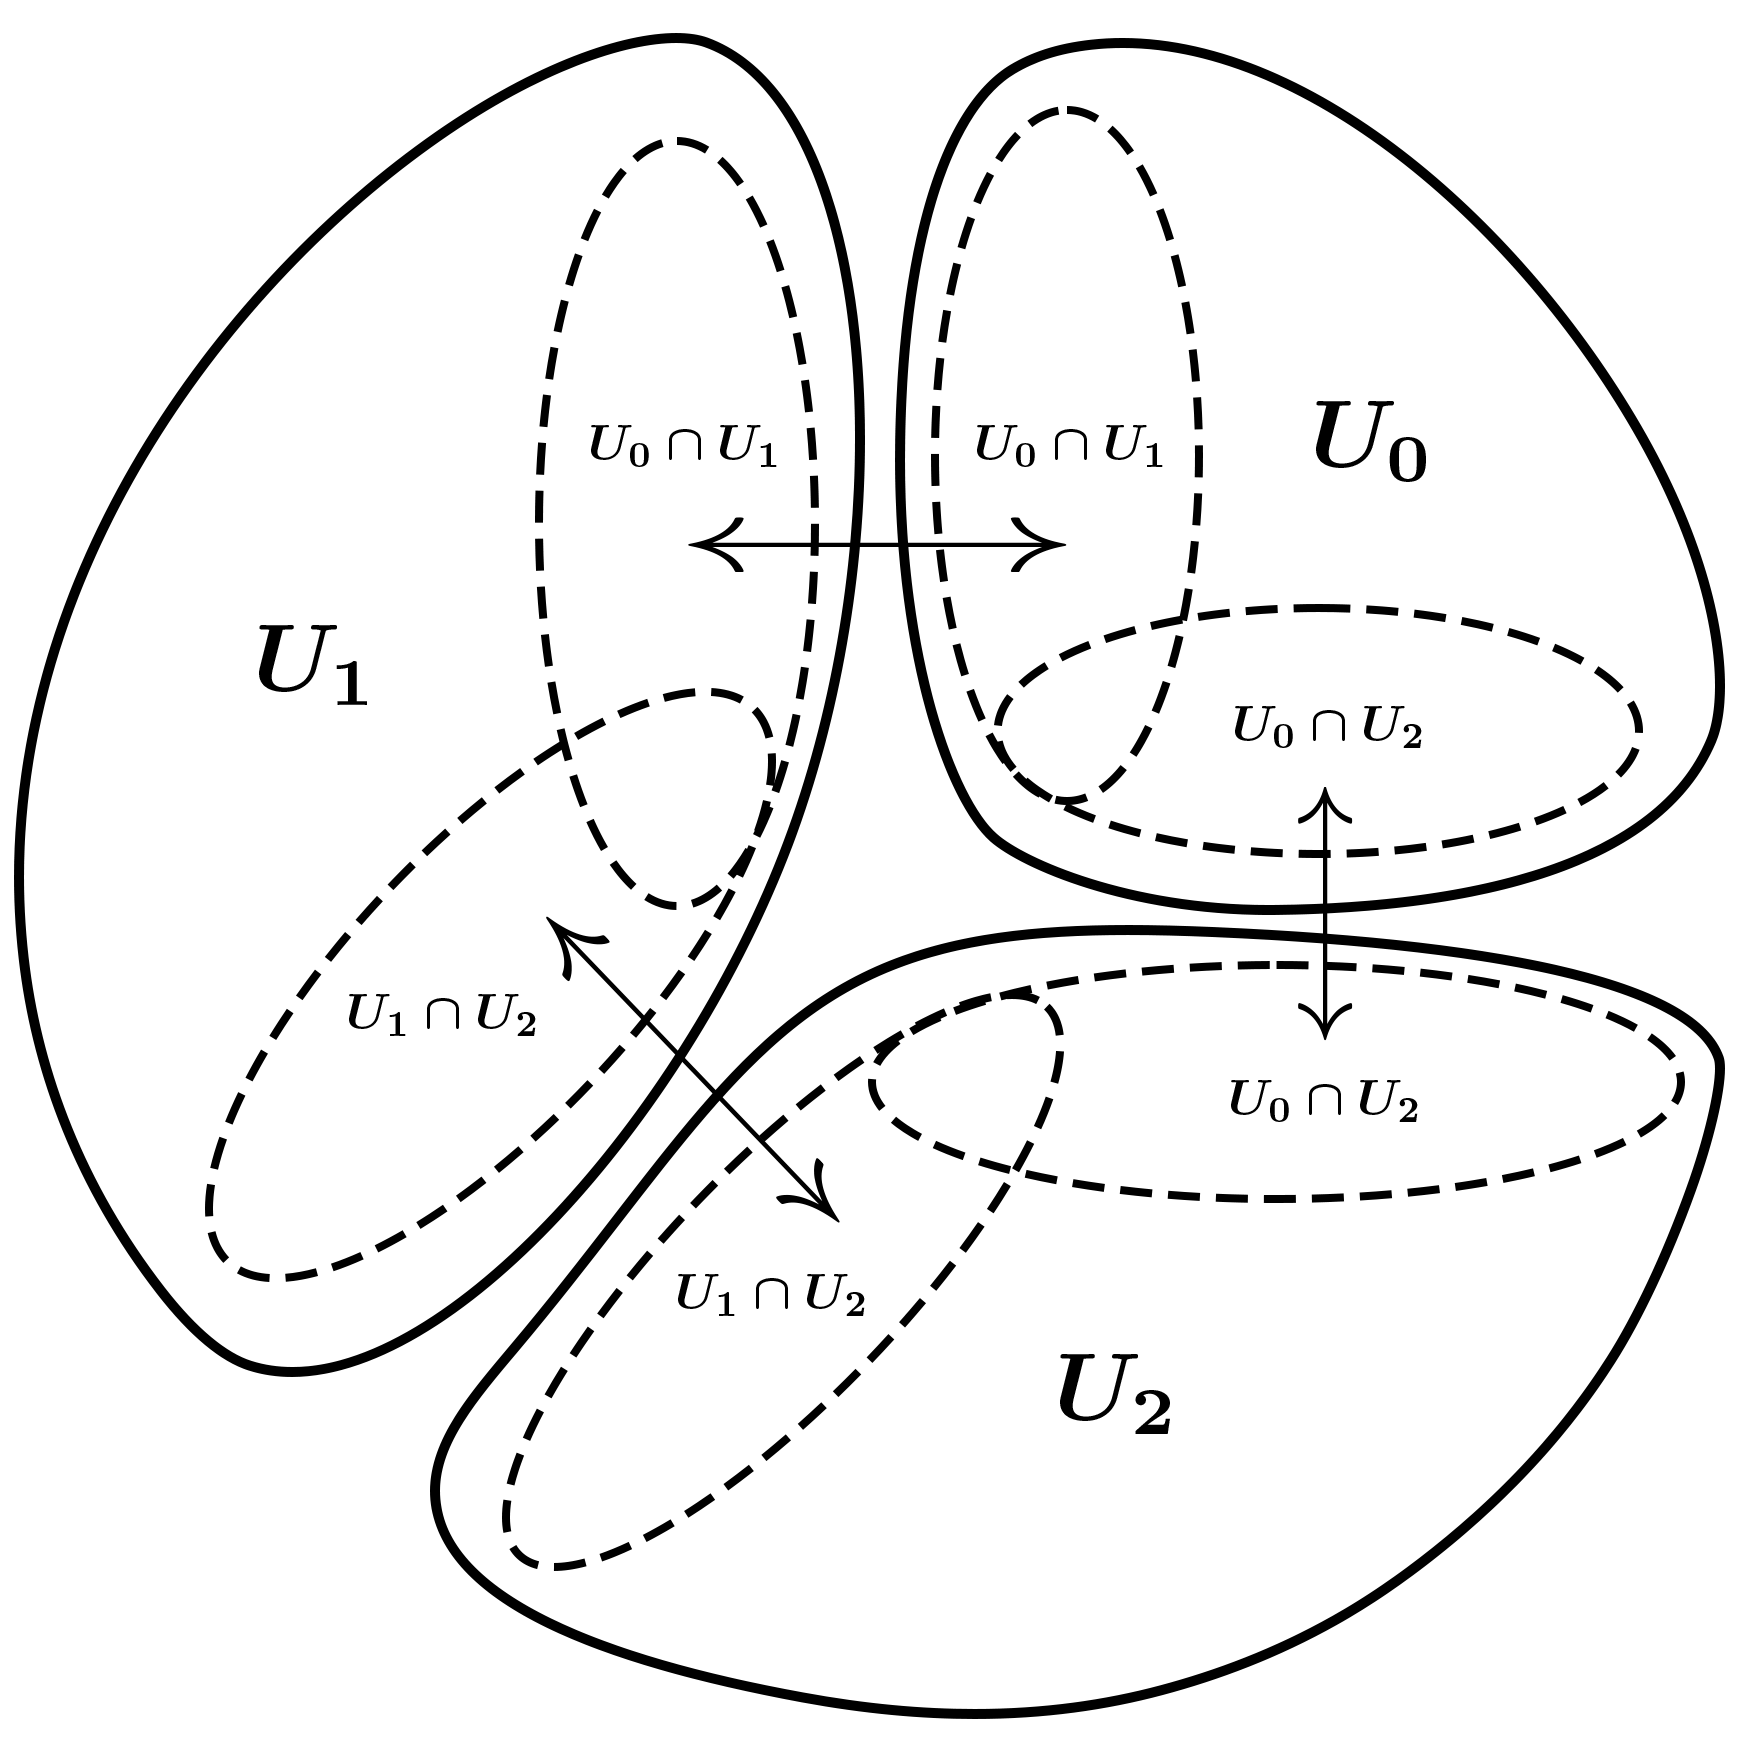
\includegraphics[width=0.5\textwidth]{affine-patches.png}
    \caption[$\mathbb{C}\mathbb{P}^2$ realised as the gluing of three affine patches $U_0, U_1$, and $U_2$.]{$\mathbb{C}\mathbb{P}^2$ realised as the gluing of three affine patches $U_0, U_1$, and $U_2$ \cite{toricfanovarieties2005}.}
    \label{fig:affine-patches-diagram}
\end{figure}

Once we have introduced homogeneous coordinates, we obtain another natural embedding of $\mathbb{R}\mathbb{P}^n$ into $\mathbb{C}\mathbb{P}^n$ by the map
\[
    \mathbb{R}\mathbb{P}^n \hookrightarrow \mathbb{C}\mathbb{P}^n \quad \quad [x_{0}, \dots, x_{n}] \mapsto [x_{0}, \dots, x_{n}] \quad \text{for} \ x_{i} \in \mathbb{R}.
\]
A point $[z] \in \mathbb{C}\mathbb{P}^n$ is called \textit{real} if any of the following equivalent conditions are satisfed:
\begin{itemize}
    \item It lies in the image of the embedding map, i.e. $[z] \in \mathbb{R}\mathbb{P}^n$.
    \item It possesses a real representative in homogeneous coordinates, i.e. $[z] = [x_{0}, \dots, x_{n}]$ for $x_{i} \in \mathbb{R}$.
    \item It is equal to its complex conjugate point, i.e. $[z] = [\bar{z}]$.
\end{itemize}
Otherwise, it is called \textit{imaginary}. Note that a real point also has imaginary representatives: for instance, $[v] = [i v]$ for any non-zero real vector $v \in \mathbb{R}^{n+1}$. Thus, the imaginary points are not simply those with an imaginary representative.

For a projective subspace $\mathbb{P}(U) \subset \mathbb{C}\mathbb{P}^n$, we define its \textit{real section} by
\[
    \mathbb{P}(U)_{\mathbb{R}} := \mathbb{P}(U \cap \mathbb{R}^{n+1}) = \mathbb{P}(U) \cap \mathbb{R}\mathbb{P}^n,
\]
which is the set of all the real points contained in $\mathbb{P}(U)$. The real section is necessarily a projective subspace, and its real dimension satisfes  $\text{dim}_{\mathbb{R}}\left(\mathbb{P}(U)_{\mathbb{R}}\right) \leq \text{dim}_{\mathbb{C}}\left(\mathbb{P}(U)\right)$ \cite{geometryII}.
Similarly, we define the \textit{complexification} of a projective subspace $\mathbb{P}(U) \subset \mathbb{R}\mathbb{P}^n$ as the complex span of its (real) points
\[
    \mathbb{P}(U)_{\mathbb{C}} := \mathbb{P}(\{ \lambda x + \gamma y \in \mathbb{C}^{n+1} : x, y \in U, \lambda, \gamma \in \mathbb{C} \}).
\]
The result of this complexification is also a projective subspace, whose complex dimension is equal to the real dimension of $\mathbb{P}(U)$ \cite{geometryII}. Thus, a projective subspace in $\mathbb{C}\mathbb{P}^n$ is \textit{real} if and only if $\mathbb{P}(U) = \mathbb{P}(U)_{\mathbb{R}}$. \par

\begin{proposition}[]
\label{thm:span-real-line}
An imaginary point $[z] \in \mathbb{C}\mathbb{P}^n$ is contained in exactly one real line, which is spanned by the points $[z]$ and $[\bar{z}]$.
\end{proposition}

\begin{proof}
The line $\ell = [z] \vee [\bar{z}]$ is a real line, since it's spanned by the two real points $[z + \bar{z}]$ and $[i(z - \bar{z})]$. If $[z]$ is contained in another real line $\tilde{\ell}$ then $z = \ell \wedge \tilde{\ell}$, which implies that it's a real point. Therefore, $[z]$ is contained in exactly one real line $\ell$.
\end{proof}

\subsection{The absolute conic of Euclidean geometry}
\label{subsec:absolute-quadrics}

\subsection{Circles on quadrics}
\label{subsec:circles-on-quadrics}

Now we are ready to prove that any (non-singular, non-degenerate) quadric except for hyperbolic paraboloids contains two circles through every point.

\begin{theorem}
\label{thm:circular-sections-hyperboloid}
Let $Q \subset \mathbb{R}^3$ be the two-sheeted hyperboloid
\begin{equation}
\label{eq:two-sheeted-alpha-beta-gamma}
Q : \frac{x^2}{\alpha} - \frac{y^2}{\beta} - \frac{z^2}{\gamma} = 1
\end{equation}
with $\alpha, \beta, \gamma > 0$ and $\gamma > \beta$. Then the circular sections of $Q$ are given by the two one-parameter families of parallel planes
\begin{equation}
\label{eq:planes-two-sheeted}
\Pi_{\pm}(\lambda_{\pm}) :\sqrt{\beta (\alpha + \gamma)} x \pm \sqrt{\alpha (\gamma - \beta)} y = \lambda_{\pm}, \quad \quad \lambda_{\pm} \in \mathbb{R} \setminus \left[-\lambda_{0}, \lambda_{0} \right]
\end{equation}
with $\lambda_{0} := \sqrt{\alpha \beta (\alpha+\beta)}$.
\end{theorem}

\begin{proof}
    We embed $\mathbb{R}^3$ into the real projective space $\mathbb{R}\mathbb{P}^3$ and further into the complex projective space $\mathbb{C}\mathbb{P}^3$, and introduce homogeneous coordinates $x_{0}, x_{1}, x_{2}$, and $x_{3}$ such that $x = x_{0} / x_{3}, y = x_{1} / x_{3}$, and $z = x_{2} / x_{3}$. Thus, we identify the plane $x_{3} = 0$ with the plane at infinity. \newline
We homogenize the affine equation of $Q$ to get
\[
    \frac{x_{0}^2}{\alpha} - \frac{x_{1}^2}{\beta} - \frac{x_{2}^2}{\gamma} - x_{3}^2 = 0.
\]
As we have shown in \hyperref[thm:span-real-line]{Thereom 1.0}, a conic contained in a plane is a circle if and only if it intersects the absolute conic at infinity
\[
    \mathcal{Z} : x_{0}^2 + x_{1}^2 + x_{2}^2 = 0, \quad x_{3} = 0
\]
in two points, also known as the circular points of the plane. Computing the intersection $Q \cap \mathcal{Z}$, we get four points at infinity in the form of two complex-conjugate solutions to the intersecting equations
\[
P_{\pm} =
\begin{bmatrix}[1.5]
\pm \sqrt{\frac{1}{\beta} - \frac{1}{\gamma}}\\
\sqrt{\frac{1}{\alpha} + \frac{1}{\gamma}}\\
i\sqrt{\frac{1}{\alpha} + \frac{1}{\beta}}\\
0
\end{bmatrix},
\quad \text{and} \quad
\overbar{P}_{\pm} =
\begin{bmatrix}[1.5]
\pm \sqrt{\frac{1}{\beta} - \frac{1}{\gamma}}\\
\sqrt{\frac{1}{\alpha} + \frac{1}{\gamma}}\\
-i\sqrt{\frac{1}{\alpha} + \frac{1}{\beta}}\\
0
\end{bmatrix}.
\]
Each complex-conjugate pair spans a real line at infinity \hyperref[thm:span-real-line]{(Proposition 2.1)}. We define $\ell_{\pm} := [P_{\pm}] \vee [\overbar{P}_{\pm}]$. The Plücker matrix of each line is given by
\begin{align*}
M_{\ell_{\pm}} &= [P_{\pm} \overbar{P}_{\pm}^{\top}] - [\overbar{P}_{\pm} P_{\pm}^{\top}]\\
&= \begin{bmatrix}
0 && 0 && \mp 2 i \sqrt{\frac{1}{\alpha} + \frac{1}{\beta}} \sqrt{\frac{1}{\beta} - \frac{1}{\gamma}} && 0\\
0 && 0 && -2 i \sqrt{\frac{1}{\alpha} + \frac{1}{\beta}} \sqrt{\frac{1}{\alpha} + \frac{1}{\gamma}} && 0\\
\pm 2 i \sqrt{\frac{1}{\alpha} + \frac{1}{\beta}} \sqrt{\frac{1}{\beta} - \frac{1}{\gamma}} && 2 i \sqrt{\frac{1}{\alpha} + \frac{1}{\beta}}\sqrt{ \frac{1}{\alpha} + \frac{1}{\gamma}} && 0 && 0\\
\end{bmatrix},
\end{align*}
which is a $4 \times 4$ skew-symmetric homogeneous matrix with rank $2$. Its two-dimensional nullspace spans the pencil of planes with the real line $\ell_{\pm}$ as its axis. Therefore, the equation of such pencil in homogeneous coordinates can be written as
\[
    \Pi_{\pm}(\lambda_{\pm}) : \sqrt{\beta (\alpha + \gamma)} x_{0} \pm \sqrt{\alpha (\gamma - \beta)} x_{1} - \lambda_{\pm} x_{3} = 0
\]
where $\lambda_{\pm}$ is the free parameter of the pencil. Since the planes from each individual family intersect in a line at infinity, they must be parallel planes. By construction, their intersection with $Q$ (if non-empty) gives all the circles contained in $Q$. \par
It remains to show for which values of $\lambda_{\pm}$ the intersection $Q \cap \Pi_{\pm}(\lambda_{\pm})$ is a non-empty intersection. For this purpose, we identify $Q$ with its Gram matrix
\[
Q =
\begin{bmatrix}
1 / \alpha && 0 && 0 && 0 \\
0 && -1 / \beta && 0 && 0 \\
0 && 0 && -1 / \gamma && 0 \\
0 && 0 && 0 && -1
\end{bmatrix},
\]
such that its corresponding quadratic form $q$ is given by $q(v) = v^{\top} Q v$. The planes of the circular sections $\Pi_{\pm}(\lambda_{\pm})$ correspond to the points
\[
p_{\pm}({\lambda_{\pm}}) =
\begin{bmatrix}[1.3]
\sqrt{\beta (\alpha + \gamma)}\\
\pm \sqrt{\alpha (\gamma - \beta)}\\
0\\
-\lambda_{\pm}
\end{bmatrix}
\]
in the dual projective space $(\mathbb{C}\mathbb{P}^3)^{*}$, and their poles with respect to $Q$ have the coordinates $Q^{-1}p_{\pm}({\lambda_{\pm}})$. Thus, $Q \cap \Pi_{\pm}(\lambda_{\pm})$ is a non-empty if and only if
\[
    q(Q^{-1}p_{\pm}({\lambda_{\pm}})) = \alpha \beta (\alpha + \gamma) - \alpha \beta (\beta - \gamma) - \lambda_{\pm}^2 \geq 0
\]
which is satisfed for $\lambda_{\pm} \in \mathbb{R} \setminus \left[-\lambda_0, \lambda_0\right]$ with $\lambda := \sqrt{\alpha \beta (\alpha+\beta)}$.
\end{proof}

\begin{figure}[H]
  \begin{subfigure}[b]{0.5\textwidth}
    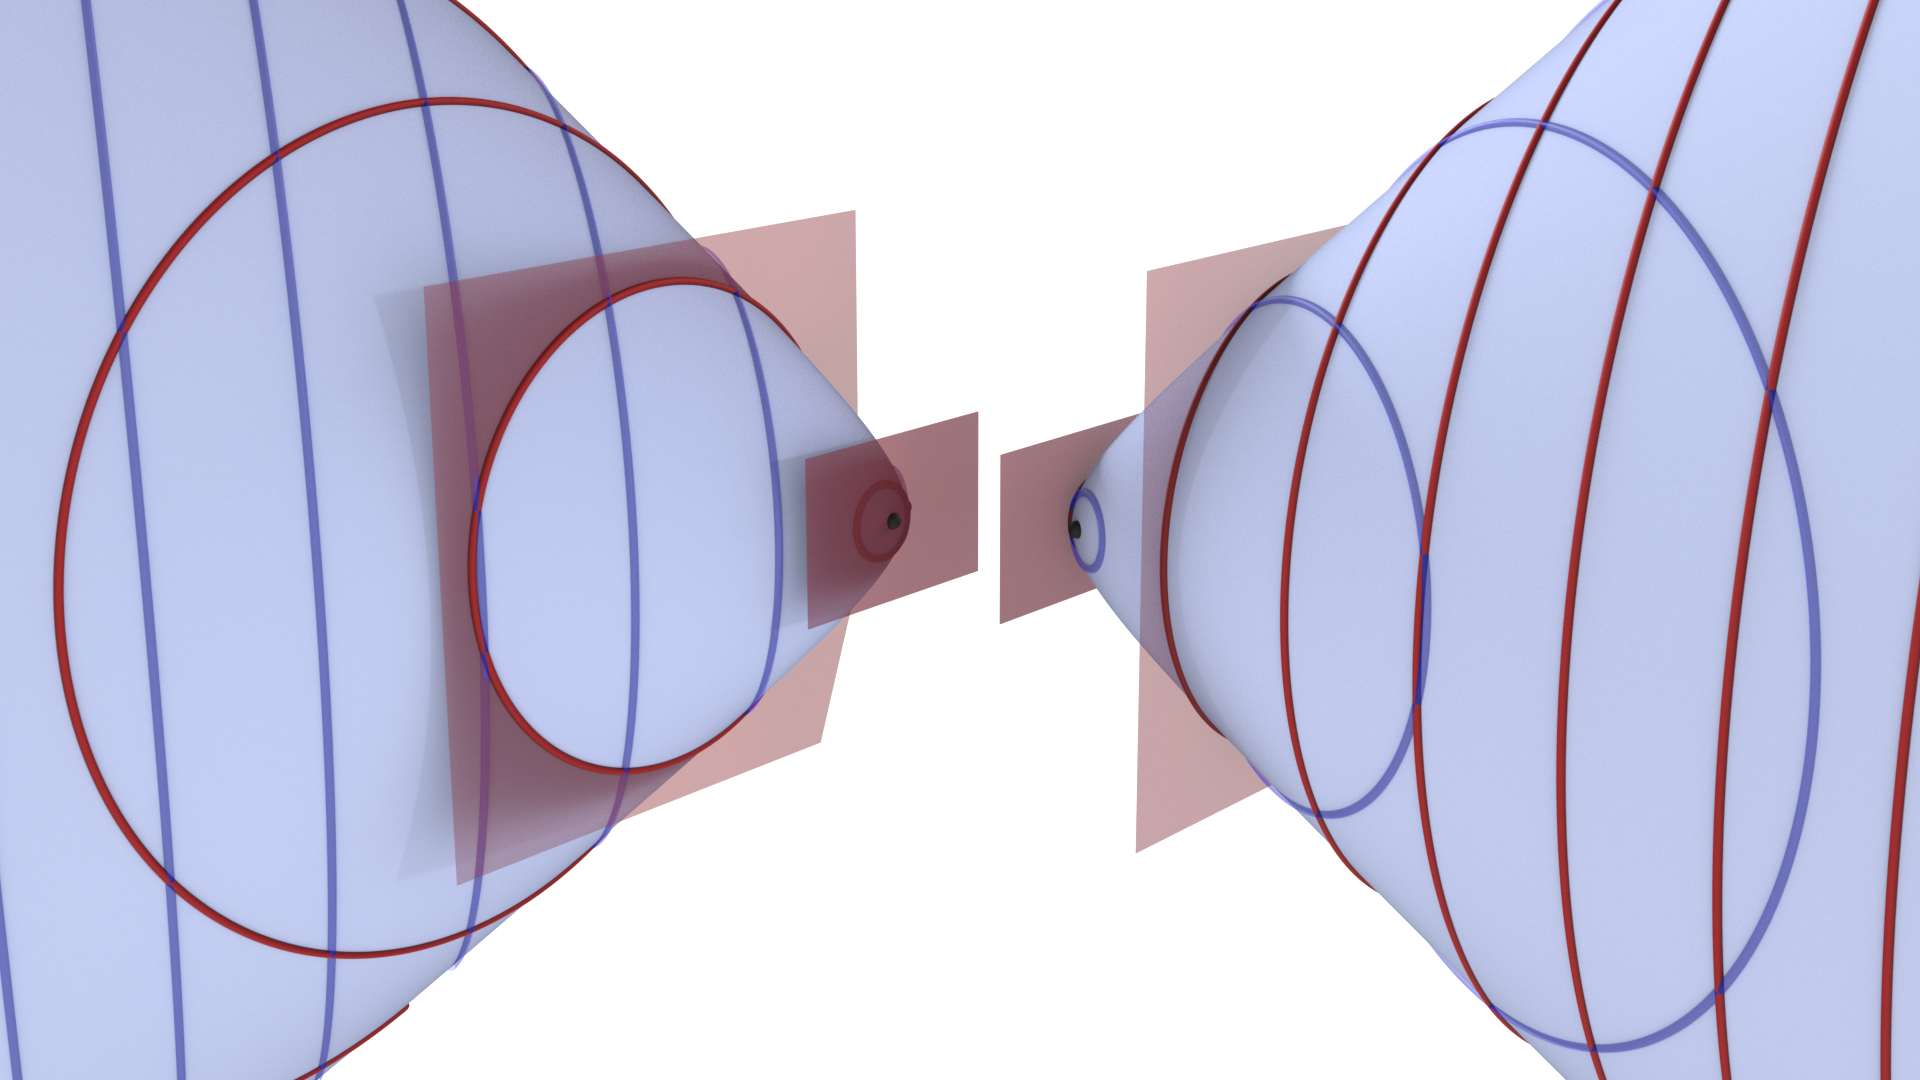
\includegraphics[width=\textwidth]{umbilics_two_sheeted_hyperboloid_red.png}
    \label{fig:two_sheeted_red}
  \end{subfigure}
  \hfill
  \begin{subfigure}[b]{0.5\textwidth}
    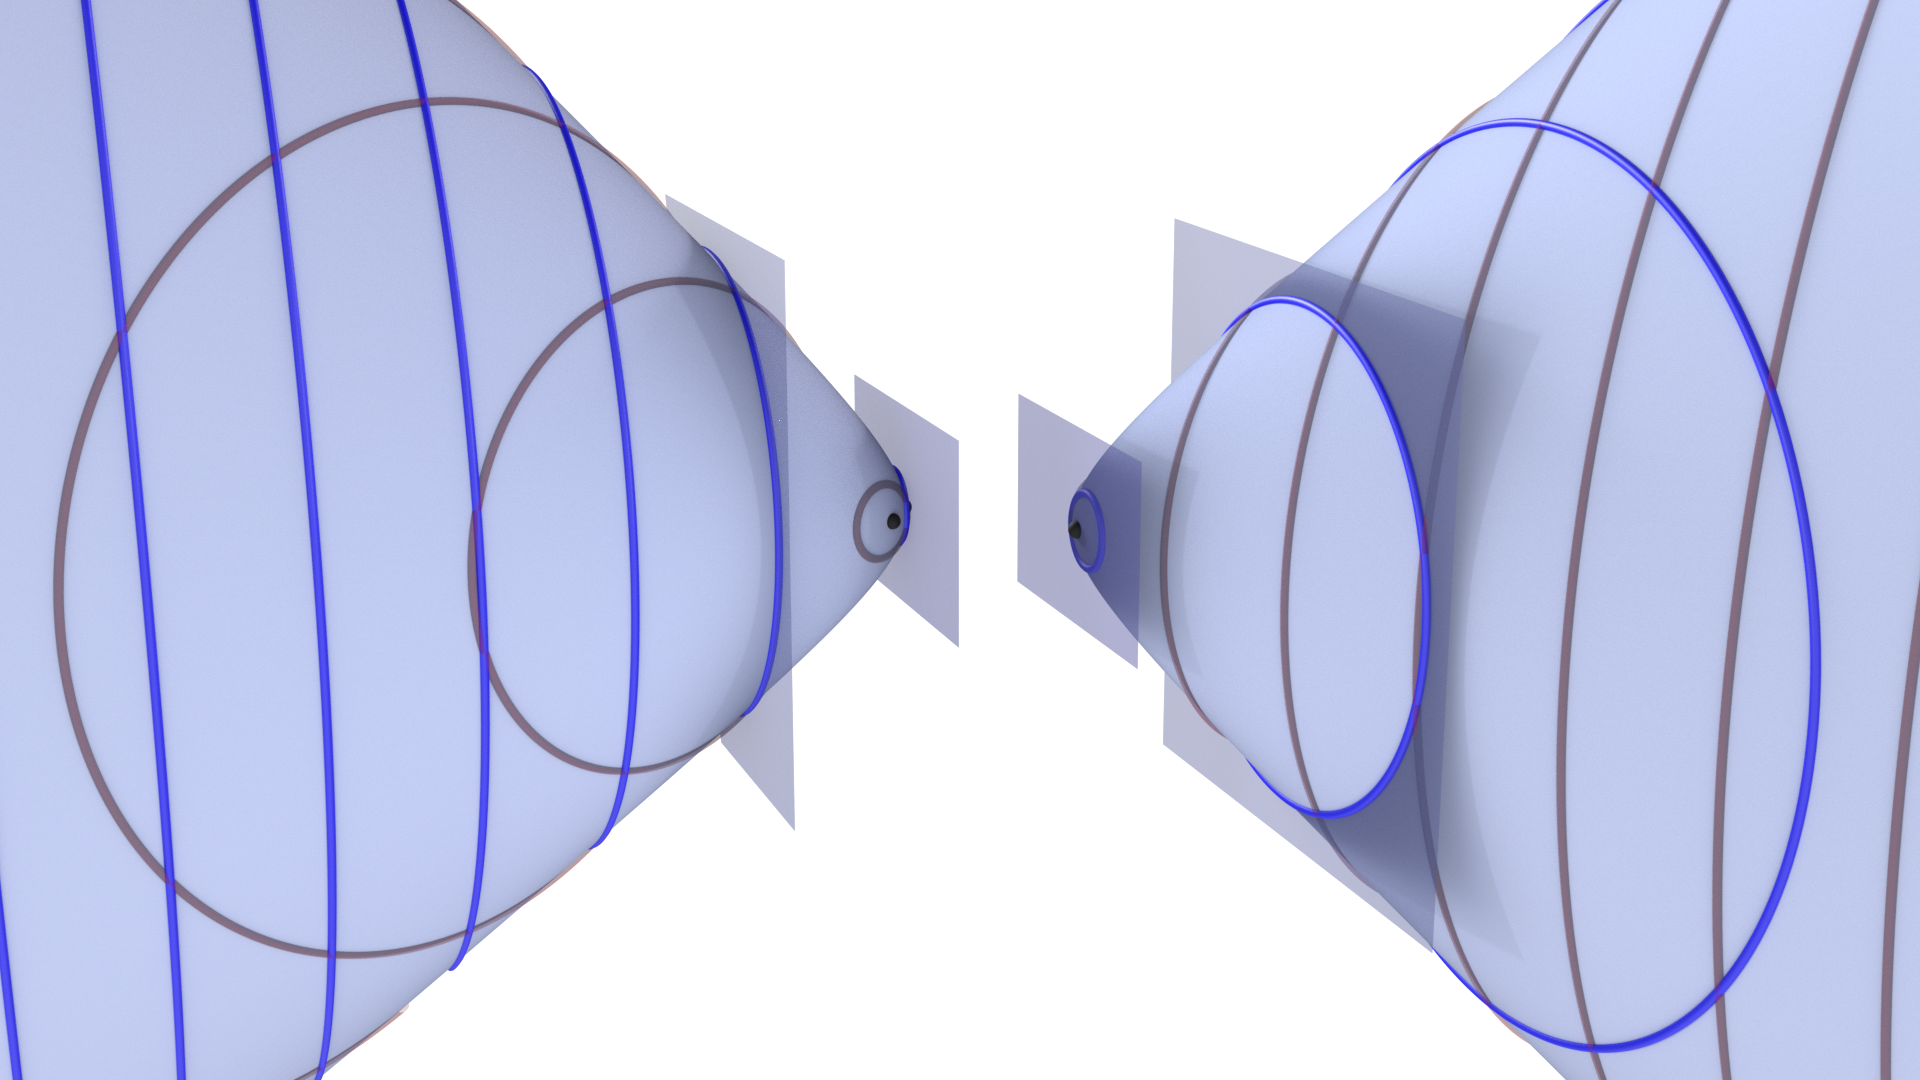
\includegraphics[width=\textwidth]{umbilics_two_sheeted_hyperboloid_blue.png}
    \label{fig:two_sheeted_blue}
  \end{subfigure}
  \caption{Two-sheeted hyperboloid carry two one-parameter families of circular sections. The planes of circular sections are parallel to the tangent planes at the umbilic points.}
\end{figure}

\begin{corollary}[]
\label{col:planes-parallel-umbilic-points}
Let $Q$ be the two-sheeted hyperboloid as given in \eqref{eq:two-sheeted-alpha-beta-gamma}. Then the planes of its circular sections \eqref{eq:planes-two-sheeted} are parallel to its tangent planes at its two umbilic points.
\end{corollary}

\begin{proof}
    Write.
\end{proof}


\begin{figure}[H]
    \centering
    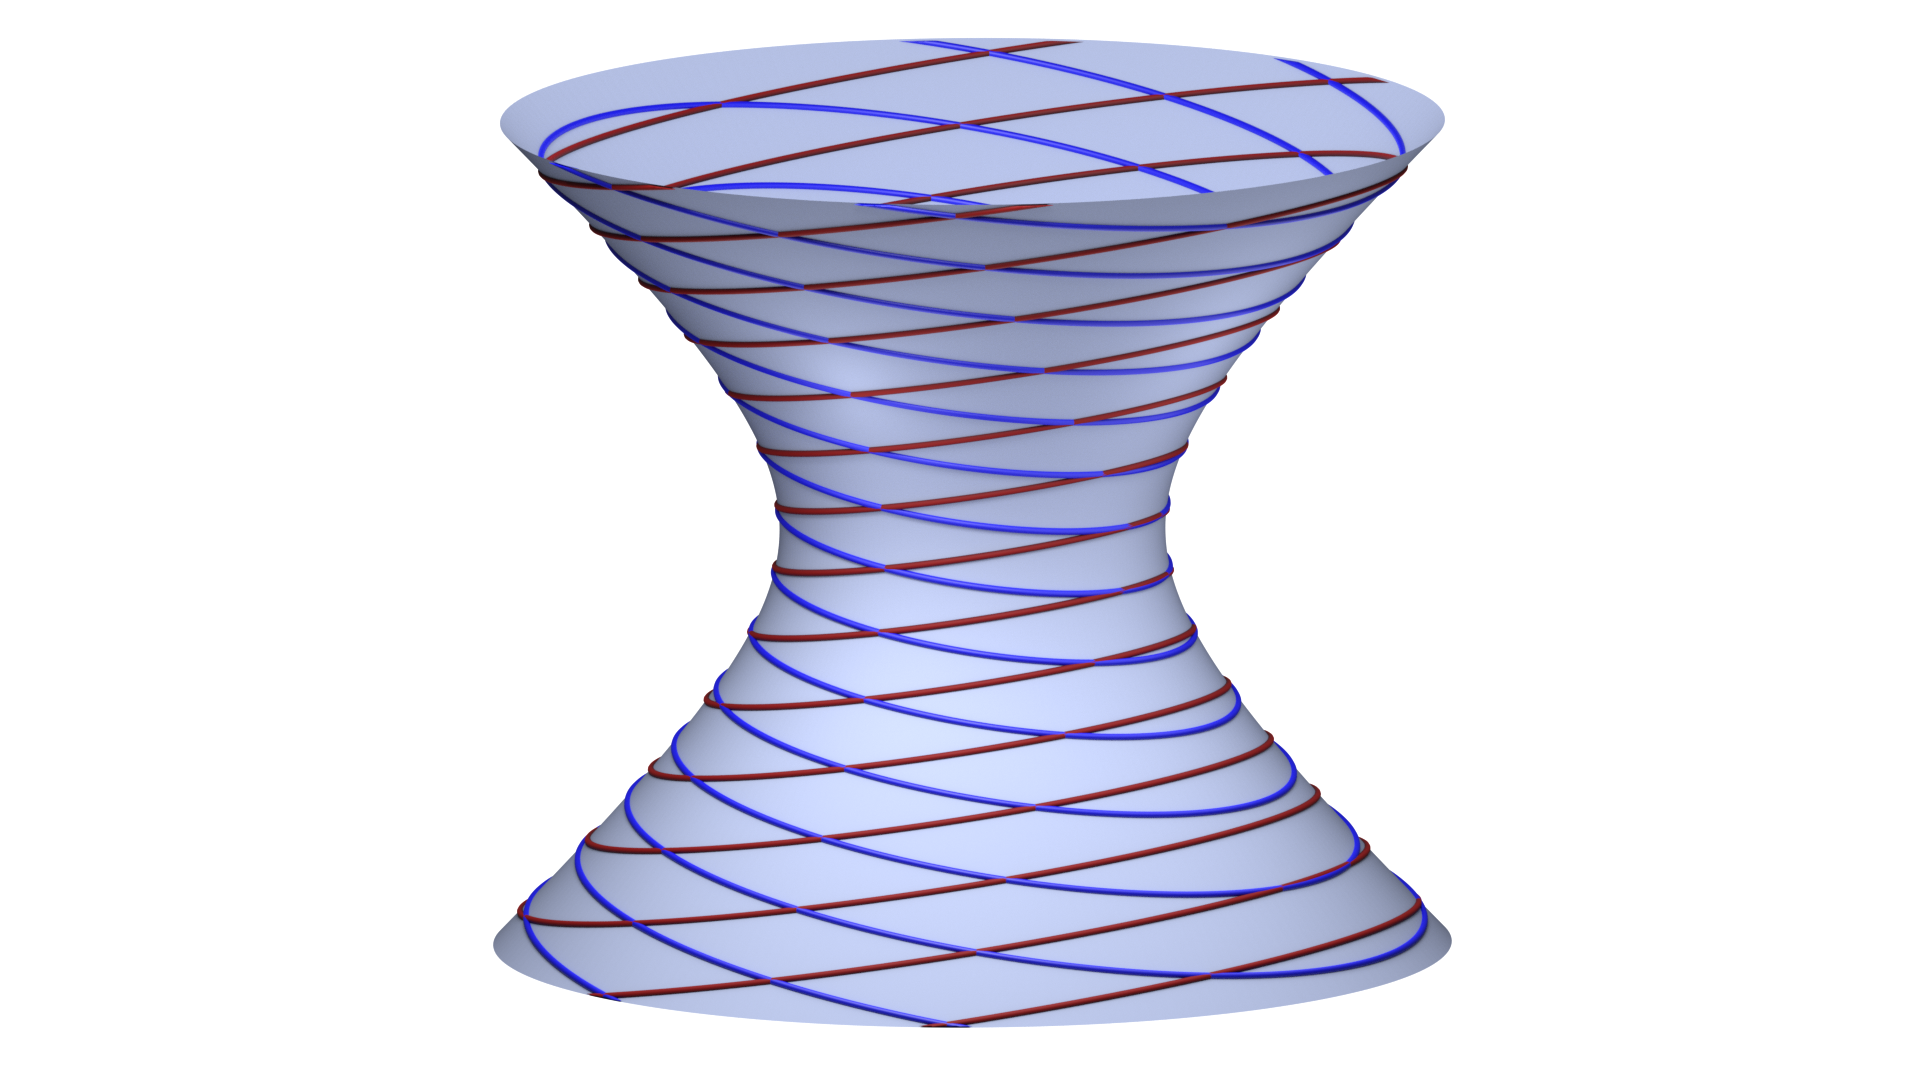
\includegraphics[width=0.8\textwidth]{circles_sections_of_one_sheeted_hyperboloid.png}
    \caption{One-sheeted hyperboloids carry two one-parameter families of circular sections.}
    \label{fig:circular_sections_one_sheeted}
\end{figure}

Using the same idea shown in the proof of \hyperref[thm:circular-sections-hyperboloid]{Thereom (2)}, we can explicity compute the circular sections of ellipsoids, one-sheeted hyperboloids and the elliptical paraboloids. We only give the resulting equations here. \par
For the ellipsoid, the equation of its two one-parameter families of parallel planes \cite{geometryIII}: \par
For the one-sheeted hyperboloid, the equation of its two one-parameter families of parallel planes: \par
For the elliptical paraboloids, the equation of its two one-parameter families of parallel planes: \par

For another proof, we can see the reference \cite{nilovSurfaceContainingLine2011}. The planes of the generating circles are parallel \cite[\textcolor{CitationColor}{\textit{Lemma~2.1}}]{nilovSurfaceContainingLine2011}, and intersect the surface only at the points of the circles \cite[\textcolor{CitationColor}{\textit{Lemma~2.6}}]{nilovSurfaceContainingLine2011}.

\pagebreak
%===========================================================
\section{Families of confocal quadrics}
\label{sec:confocal-quadrics}

\begin{definition}[]
\label{def:confocal-quadrics}
In Euclidean geometry, two quadrics in $\mathbb{R}^3$ are \textit{confocal}, sometimes also referred to as \textit{homofocal}, if they have common axes and intersect each plane of symmetry along confocal conics.
\end{definition}

\begin{figure}[H]
    \centering
    
\includegraphics[width=0.5\textwidth]{TU-Berlin-Logo.png}
    \caption{TO BE ADDED}
    \label{fig:figgg}
\end{figure}

Nondegenerate families of confocal quadrics come in two types: ellipsoids, hyperboloids of one sheet, and hyperboloids of two sheets; and downward-pointing elliptical paraboloids, hyperbolic paraboloids, and upward-pointing elliptic paraboloids. For the remaining sections, the term \textit{confocal quadrics} will refer only to the first type, i.e. a family of confocal ellipsoids, hyperboloids of one sheet, and hyperboloids of two sheets. We briefly mention confocal paraboloids in \hyperref[subsec:confocal-paraboloids]{Section 10.1}.\par

Let $a, b, c \in \mathbb{R}$ with $a > b > c > 0$ and consider a non-parabolic quadric in normal form
\[
    \frac{x^2}{a} + \frac{y^2}{b} + \frac{z^2}{c} = 1.
\]
Then any quadric confocal with it must necessarily be in normal form
\[
    \frac{x^2}{\tilde{a}} + \frac{y^2}{\tilde{b}} + \frac{z^2}{\tilde{c}} = 1
\]
with $\tilde{a} > \tilde{b} > \tilde{c} > 0$, and the differences between the fixed parameters of each quadric must all be equal, i.e.
\[
    a - b = \tilde{a} - \tilde{b}, \quad a - c = \tilde{a} - \tilde{c}, \ \text{ and } \  b - c = \tilde{b} - \tilde{c}.
\]
This motivates the following definition \cite{geometryIII}:

\begin{definition}[]
\label{def:family-of-confocal-quadrics}
Let $a, b, c \in \mathbb{R}$ with $a > b > c > 0$. Then the one-parameter family of quadrics given by
\[
    Q_{\lambda} := \left\{ (x, y, z) \in \mathbb{R}^3 : \frac{x^2}{a + \lambda} + \frac{y^2}{b + \lambda} + \frac{z^2}{c + \lambda} = 1 \right\}, \quad \lambda \in \mathbb{R}
\]
is called a family of confocal quadrics.
\end{definition}

Any triple of real numbers $a > b > c > 0$ divides the real line into four segements, and we can recover the subfamilies of quadrics of different signatures in the confocal family accordingly:

\begin{itemize}[label=$\blacktriangleright$]
    \item If $\lambda < -a$, then $Q_{\lambda}$ has no real points, or is \enquote{purely imaginary}.
    \item If $\lambda \in (-a, -b)$, then $Q_{\lambda}$ is a one-parameter family of confocal two-sheeted hyperboloids.
    \item If $\lambda \in (-b, -c)$, then $Q_{\lambda}$ is a one-parameter family of confocal one-sheeted hyperboloids.
    \item If $\lambda > -c$, then $Q_{\lambda}$ is a one-parameter family of confocal ellipsoids. \par
\end{itemize}

\begin{theorem}[]
\label{thm:fill-up-euclidean-space}
For every point $(x, y, z) \in \mathbb{R}^3$ with $x \cdot y \cdot z \neq 0$, i.e. a point not on the standard coordinate planes, there passes exactly one ellipsoid, one one-sheeted hyperboloid, and one two-sheeted hyperboloid from the confocal family $Q_{\lambda}$.
\end{theorem}

\begin{proof}
    Let $a, b, c \in \mathbb{R}$ be the fixed parameters of the confocal family $Q_{\lambda}$ with $a > b > c > 0$. Given a point $(x, y, z) \in \mathbb{R}^3$, and clearing the denominators of the confocal quadrics equation
\[
    \frac{x^2}{a + \lambda} + \frac{y^2}{b + \lambda} + \frac{z^2}{c + \lambda} = 1,
\]
we see that it's a third degree polynomial equation in $\lambda$. It has three real roots $u_{1}, u_{2}$, and $u_{3}$ which can be solved for explicitly, however for our purposes it's enough to note that the three roots lie in the intervals
\[
    -a < u_{1} < -b < u_{2} < -c < u_{1}
\]
by looking at the qualitative behavior of the function
\[
    \lambda \mapsto \frac{x^2}{a + \lambda} + \frac{y^2}{b + \lambda} + \frac{z^2}{c + \lambda}
\]
over $\mathbb{R}$ [Figure ~\ref{fig:plot}].
\end{proof}

\begin{figure}[H]
    \centering
    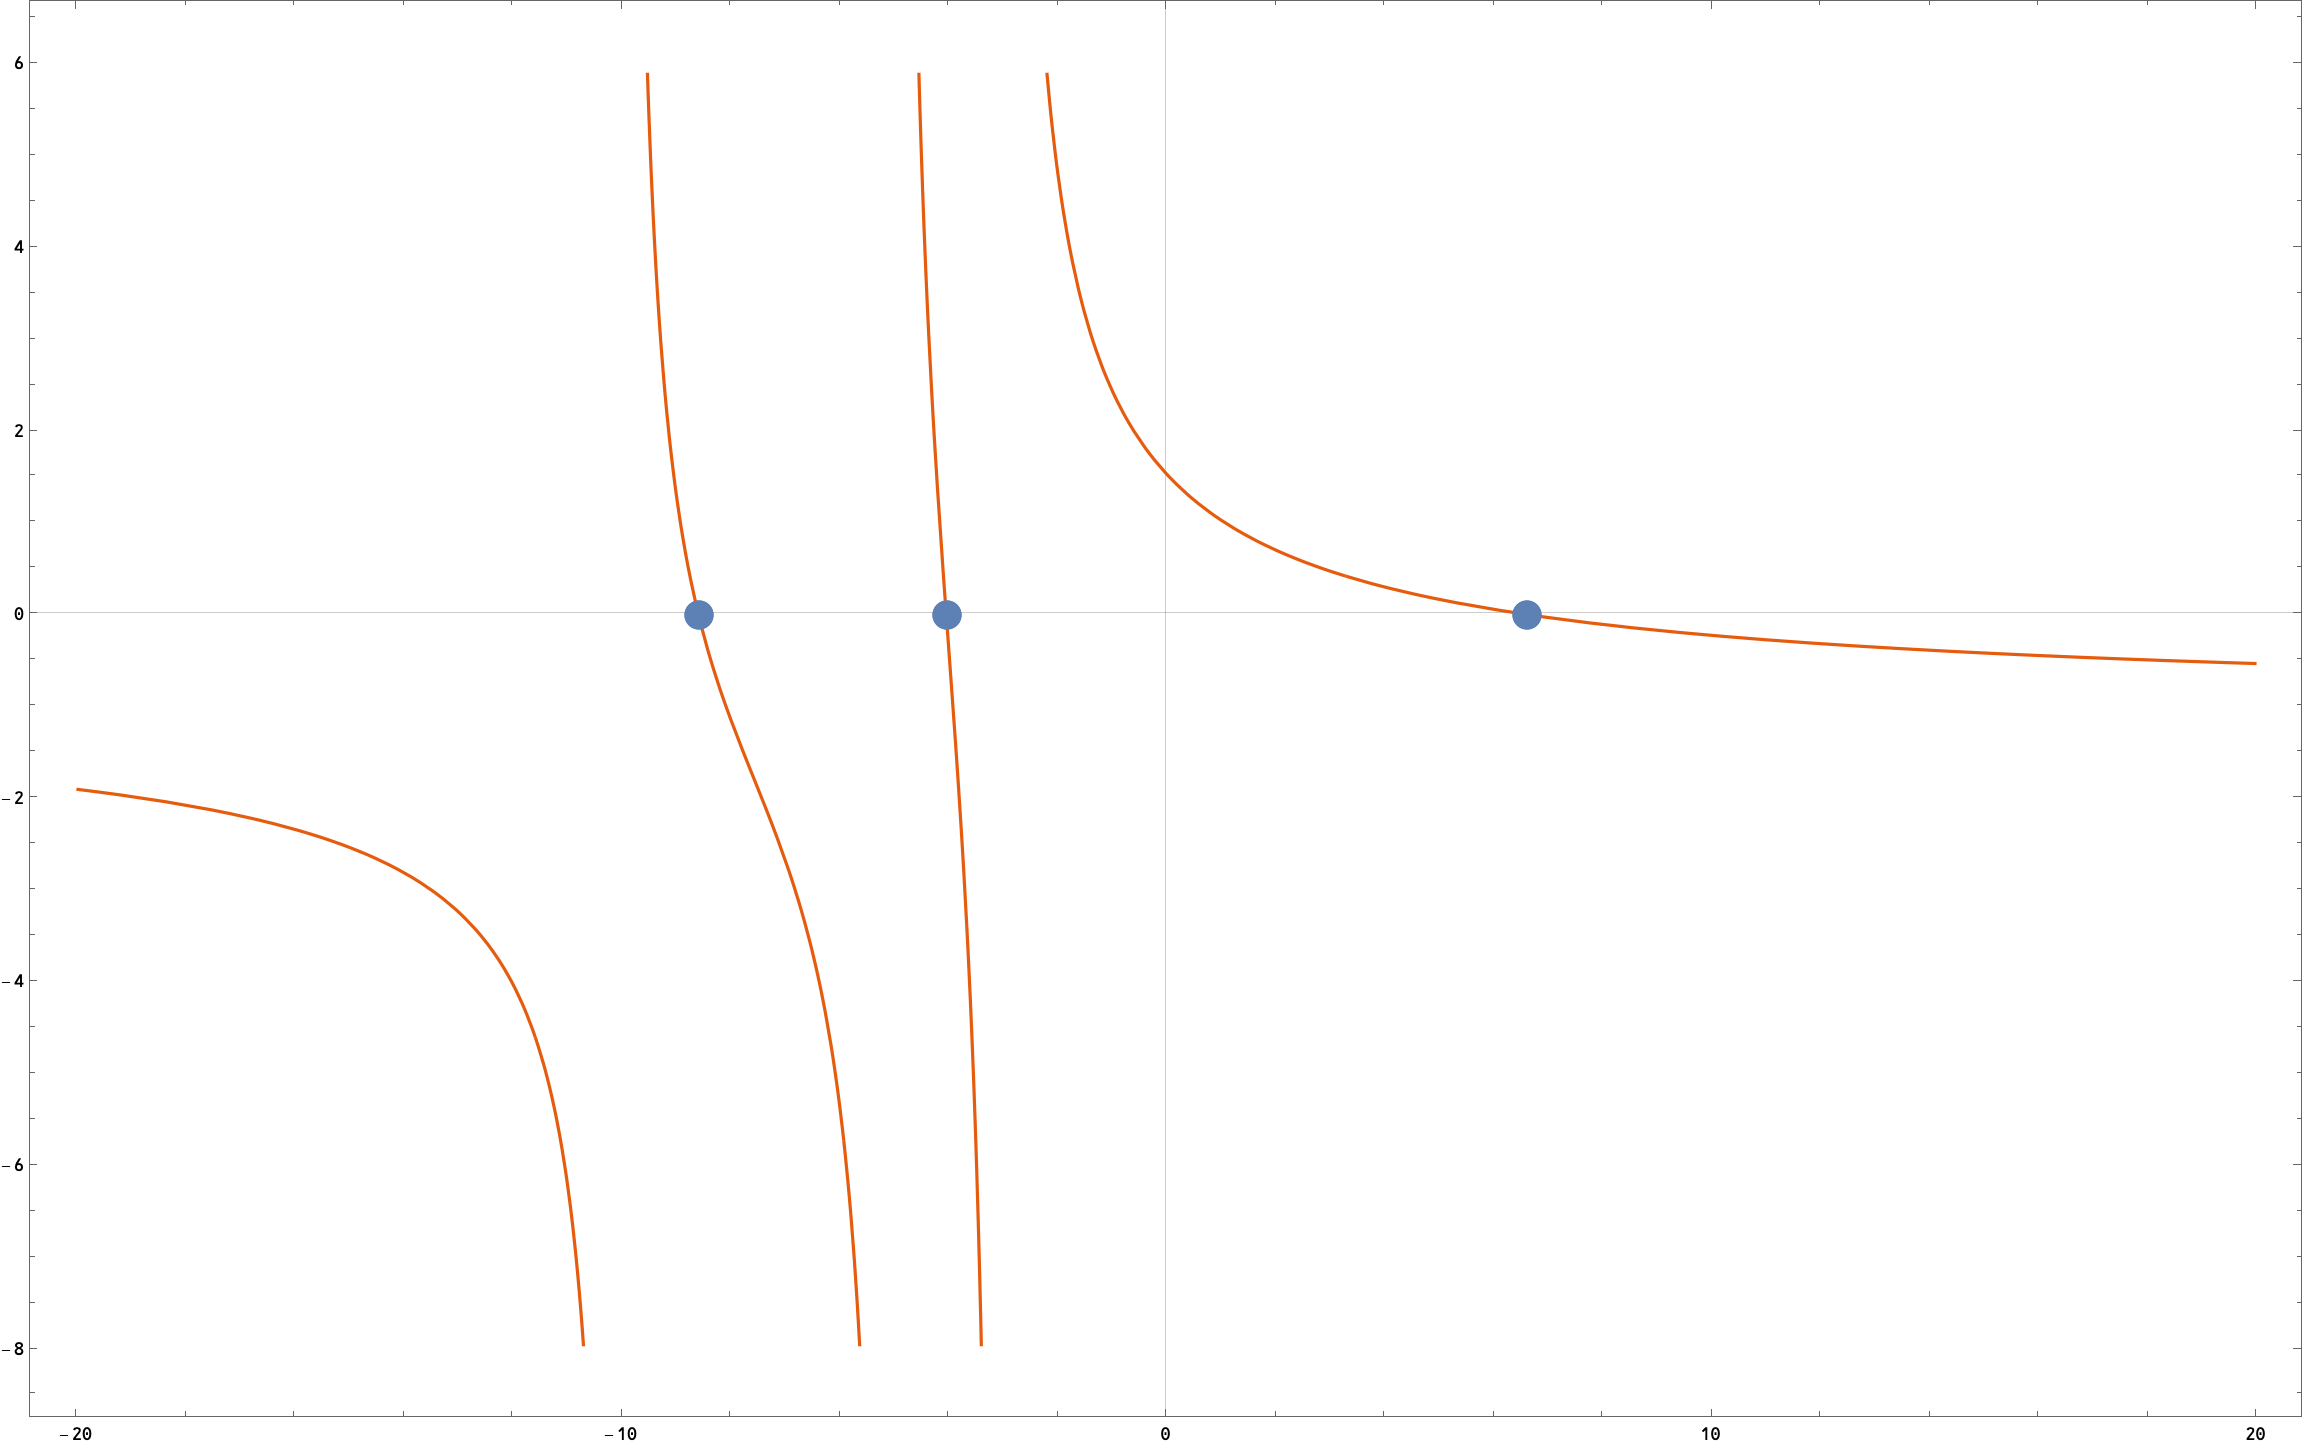
\includegraphics[width=1.0\textwidth]{graph-for-proof.png}
    \label{fig:graph-for-proof}
    \caption[A plot of the real-valued function $\lambda \mapsto \frac{x^2}{a + \lambda} + \frac{y^2}{b + \lambda} + \frac{z^2}{c + \lambda}$]{The function $\lambda \mapsto \frac{x^2}{a + \lambda} + \frac{y^2}{b + \lambda} + \frac{z^2}{c + \lambda}$ plotted for some $(x_0, y_0, z_0) \in \mathbb{R}^3$, $a = 10.0$, $b = 5.0$, and $c = 3.0$.}
    \label{fig:plot}
\end{figure}

Any triple of confocal quadrics of different signatures meet orthogonally in a unique point $(x, y, z)$ in each octant of $\mathbb{R}^3$. Due to the orthogonality of their curves of intersection, if we parameterize an individual quadric in a particular manner using the confocal family then its two families of coordinate lines are lines of curvature. We elaborate these interesting properties in the next few theorems.

\subsection{Confocal Coordinates}
\label{subsec:confocal-coordinates}

\subsection{Lines of curvature on confocal quadrics}
\label{subsec:curvature-lines-on-quadrics}
\pagebreak
%===========================================================
\section{Diagonally related nets on surfaces}
\label{sec:diagonally-related-nets}

We start by defining nets on surfaces. Mutually diagonal nets on surfaces were introduced in \cite{MutuallyDiagonalNets2019}.

\begin{definition}[]
\label{def:nets-on-surfaces}
A net $\mathcal{N}$ on a surface $\Sigma$ is a pair of one-parameter families of curves on $\Sigma$, such that for every point on $\Sigma$ there exists exactly one curve from each of the two families through that point.
\end{definition}

\begin{remark}[]
\label{rm:label}
Let $\mathcal{N} = \left( (\alpha_{s_{1}})_{s_{1} \in I_1}, (\beta_{s_{2}})_{s_{2} \in I_2} \right)$ be a net on a surface
$\Sigma$, and $P$ a point on the surface then there exists a unique pair $(s_{1}, s_{2}) \in I_{1}\times I_{2}$ such that
\[
    P = \alpha_{s_1} \cap \beta_{s_2}
\]
We call $(s_1, s_2)$ the \textit{coordinates of the point $P$ with respect to the net $\mathcal{N}$}. Note that these coordinates alone do not uniquely determine the points on the surface, especially that we don't assume that each two curves from different families of $\mathcal{N}$ intersect in one unique point. However, the net together with a specific parameterization of its curves uniquely determine the points of the surface.
\end{remark}

\begin{example}
\label{ex:coordinate-lines-form-net-on-surfaces}
Let $\varphi : I_{1} \times I_{2} \subset \mathbb{R}^2 \to \mathbb{R}^3$ be a parameterization of a surface. Then its
coordinate lines, i.e. the curves
\begin{align*}
    \varphi_{u_0} : I_{2} \to \mathbb{R}^3 &\quad \quad \varphi_{u_0}(v) = \varphi(u_0, v), \text{ and} \\
    \varphi_{v_0} : I_{1} \to \mathbb{R}^3 &\quad \quad \varphi_{v_0}(u) = \varphi(u, v_0)
\end{align*}
defined for each fixed $u_{0} \in I_1, v_{0} \in I_2$ constitute a net on the surface $\varphi\left( I_1 \times I_{2}
\right) \subset \mathbb{R}^3$.
\end{example}

\begin{example}
\label{ex:circular-sections-form-nets-on-quadrics}
In \hyperref[sec:circular-sections-of-quadrics]{Section Two} we proved that quadrics contain two circles through each point. Thus, the circular sections quadrics form a net on quadrics.
\end{example}

\begin{figure}[H]
  \begin{subfigure}[b]{0.5\textwidth}
    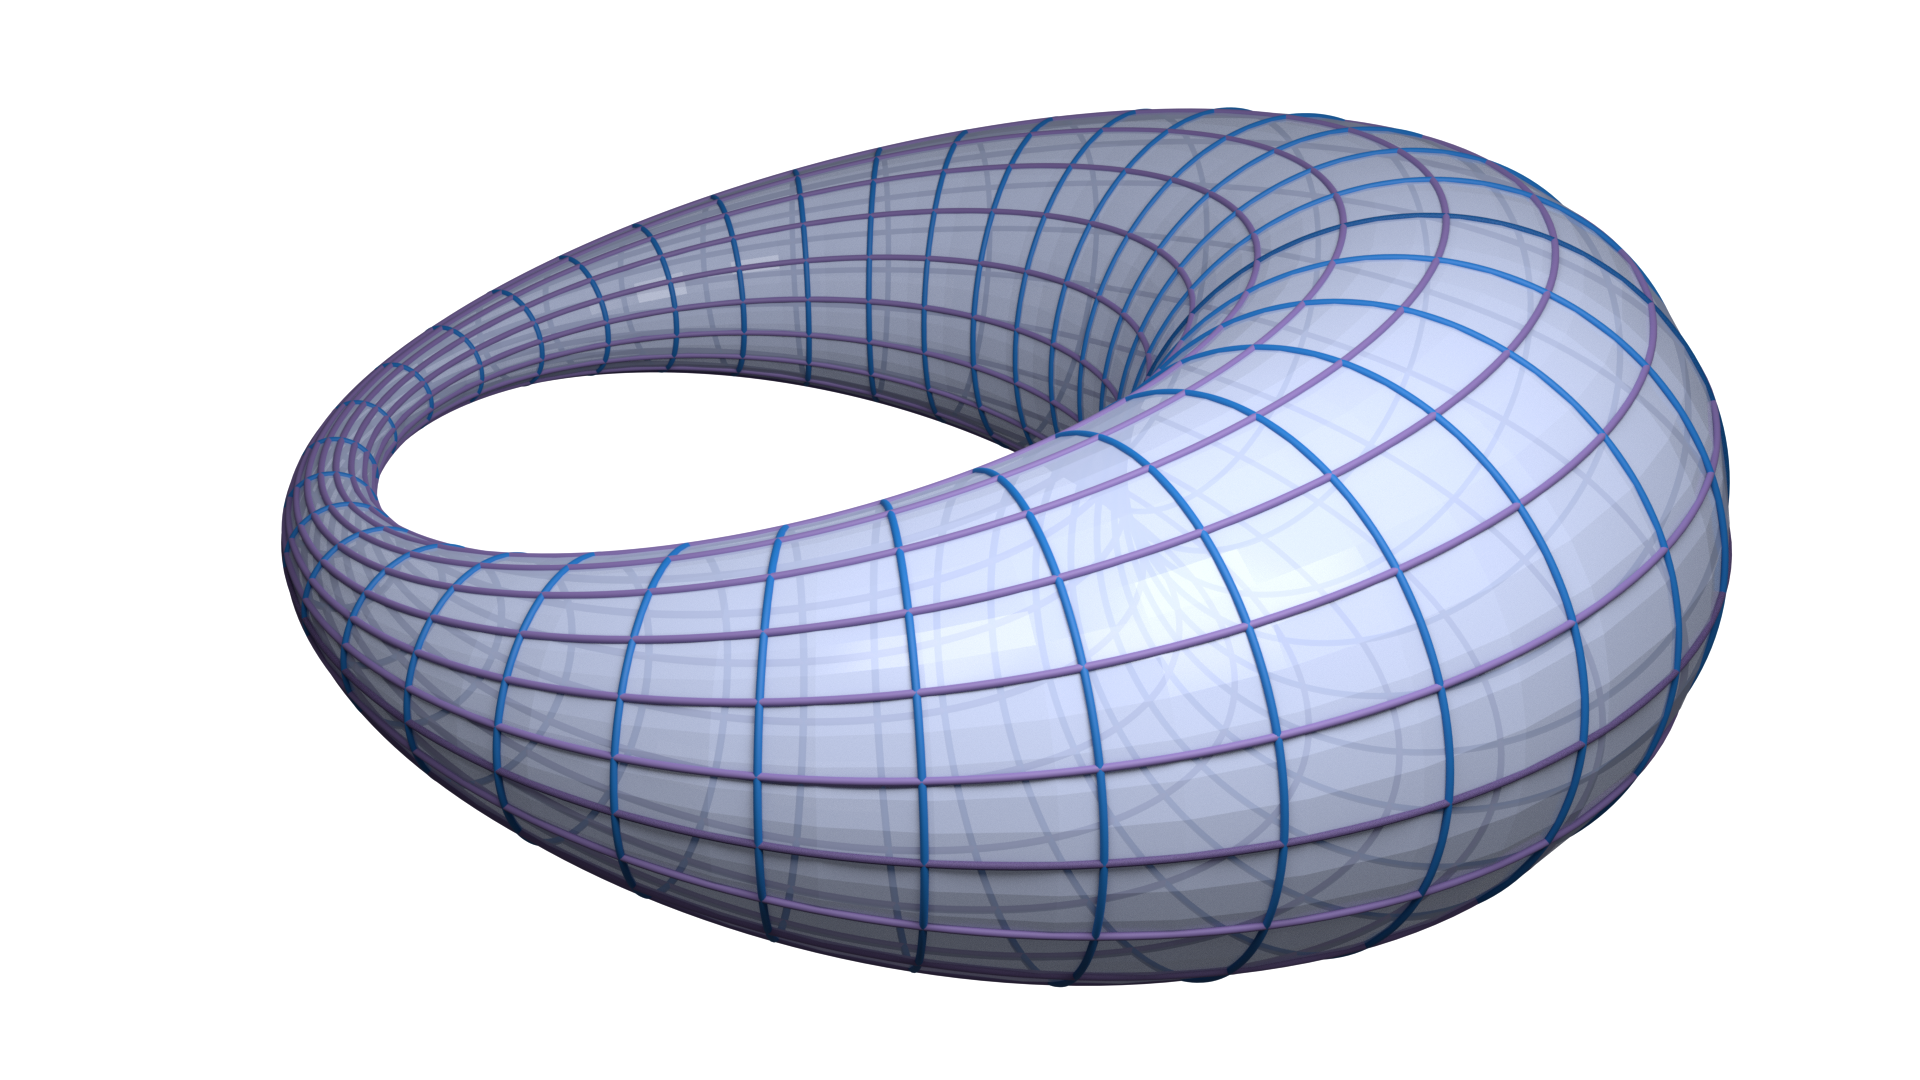
\includegraphics[width=\textwidth]{Dupin-net.png}
    \caption{ellipto-hyperbolic}
    \label{fig:ellipto-hyperbolic-cyclides}
  \end{subfigure}
  \hfill
  \begin{subfigure}[b]{0.5\textwidth}
    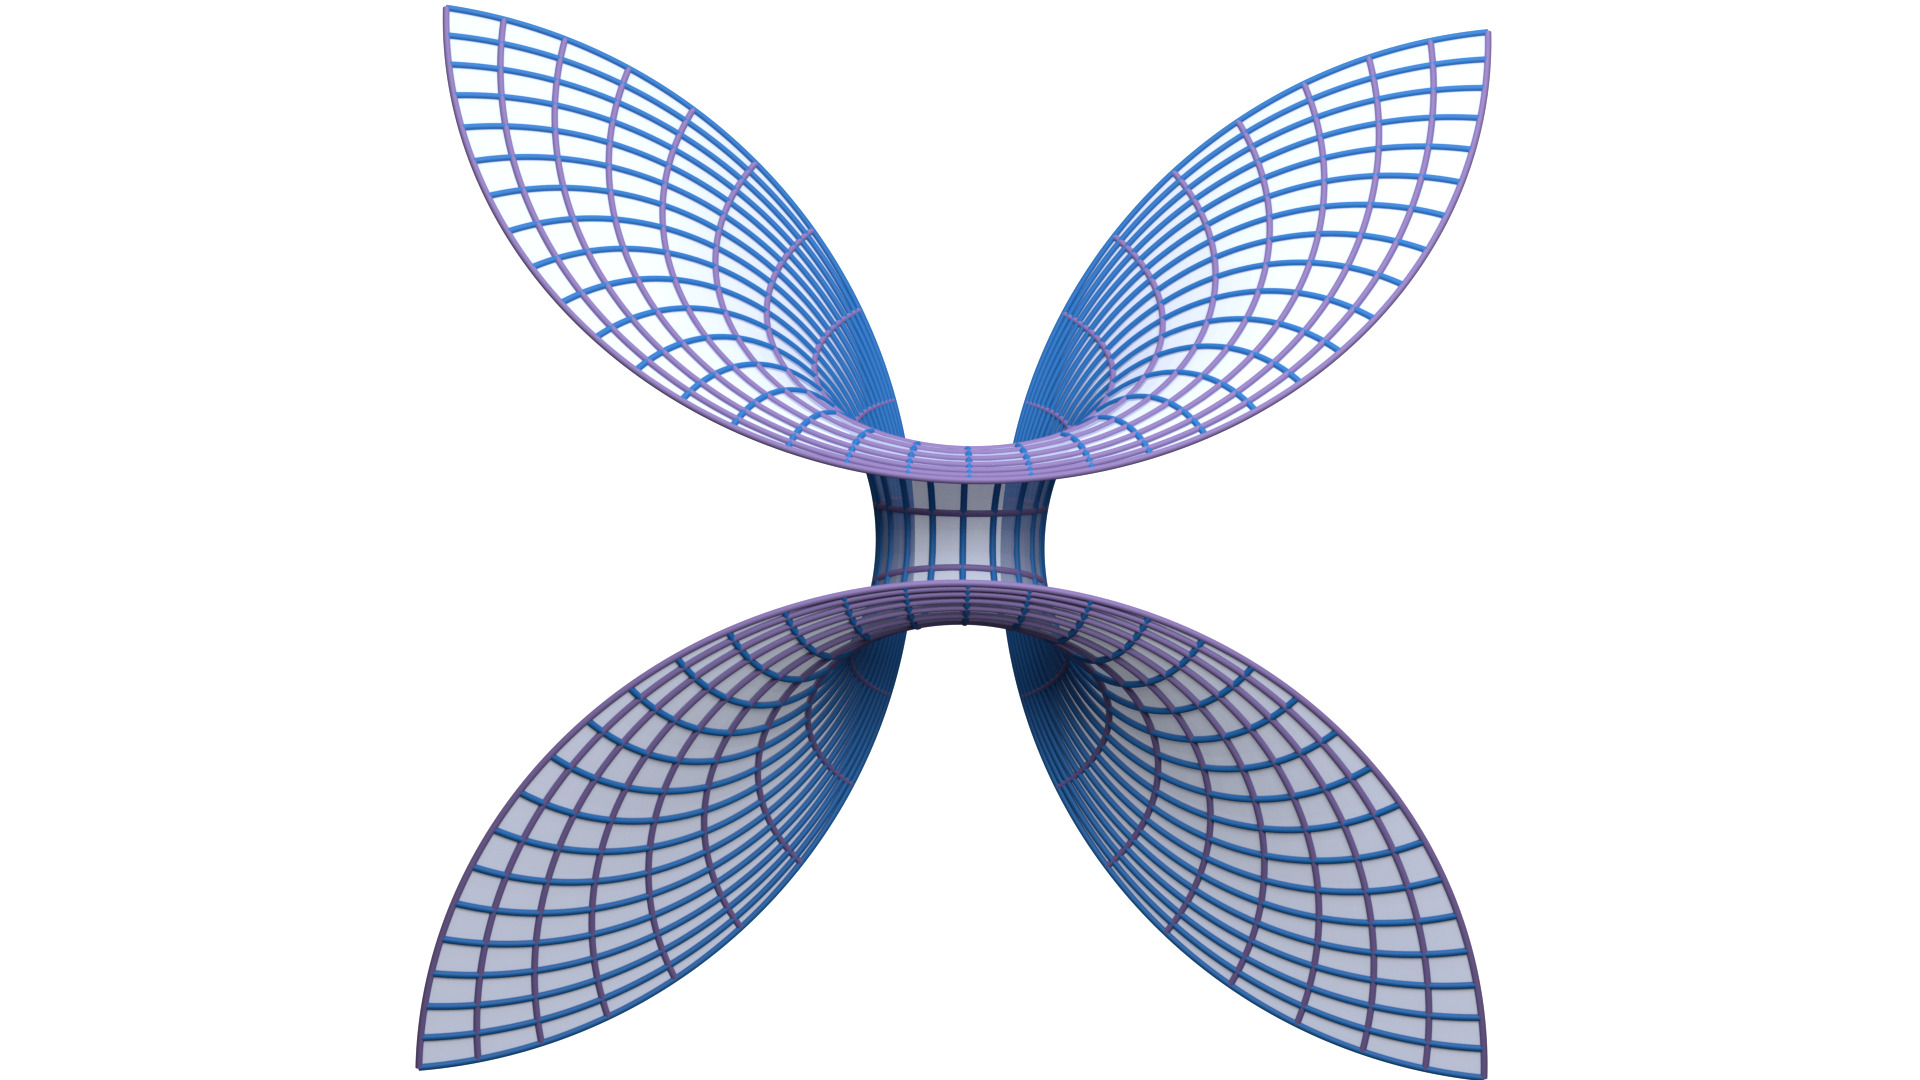
\includegraphics[width=\textwidth]{Dupin-net-2.png}
    \caption{parabolic}
    \label{fig:parabolic-cyclides}
  \end{subfigure}
  \caption{Dupin Cyclides}
\end{figure}

\begin{definition}[Diagonally related nets on surfaces]
\label{def:diag-nets-on-surfaces}
Let $\mathcal{N}_{1}$ and $\mathcal{N}_{2}$ be two nets on a surface $\Sigma$. Then $\mathcal{N}_{2}$ is called diagonal
to $\mathcal{N}_{1}$ if the following condition is satisfied whenever any four curves of $\mathcal{N}_{1}$ form a
(combinatorial) quadrilateral: \newline
\begin{mathbox}{}
If one pair of opposite vertices is connected by a curve from $\mathcal{N}_{2}$, then the other pair of opposite vertices is connected by a curve from $\mathcal{N}_{1}$.
\end{mathbox}
\end{definition}

\begin{figure}[H]
    \centering
    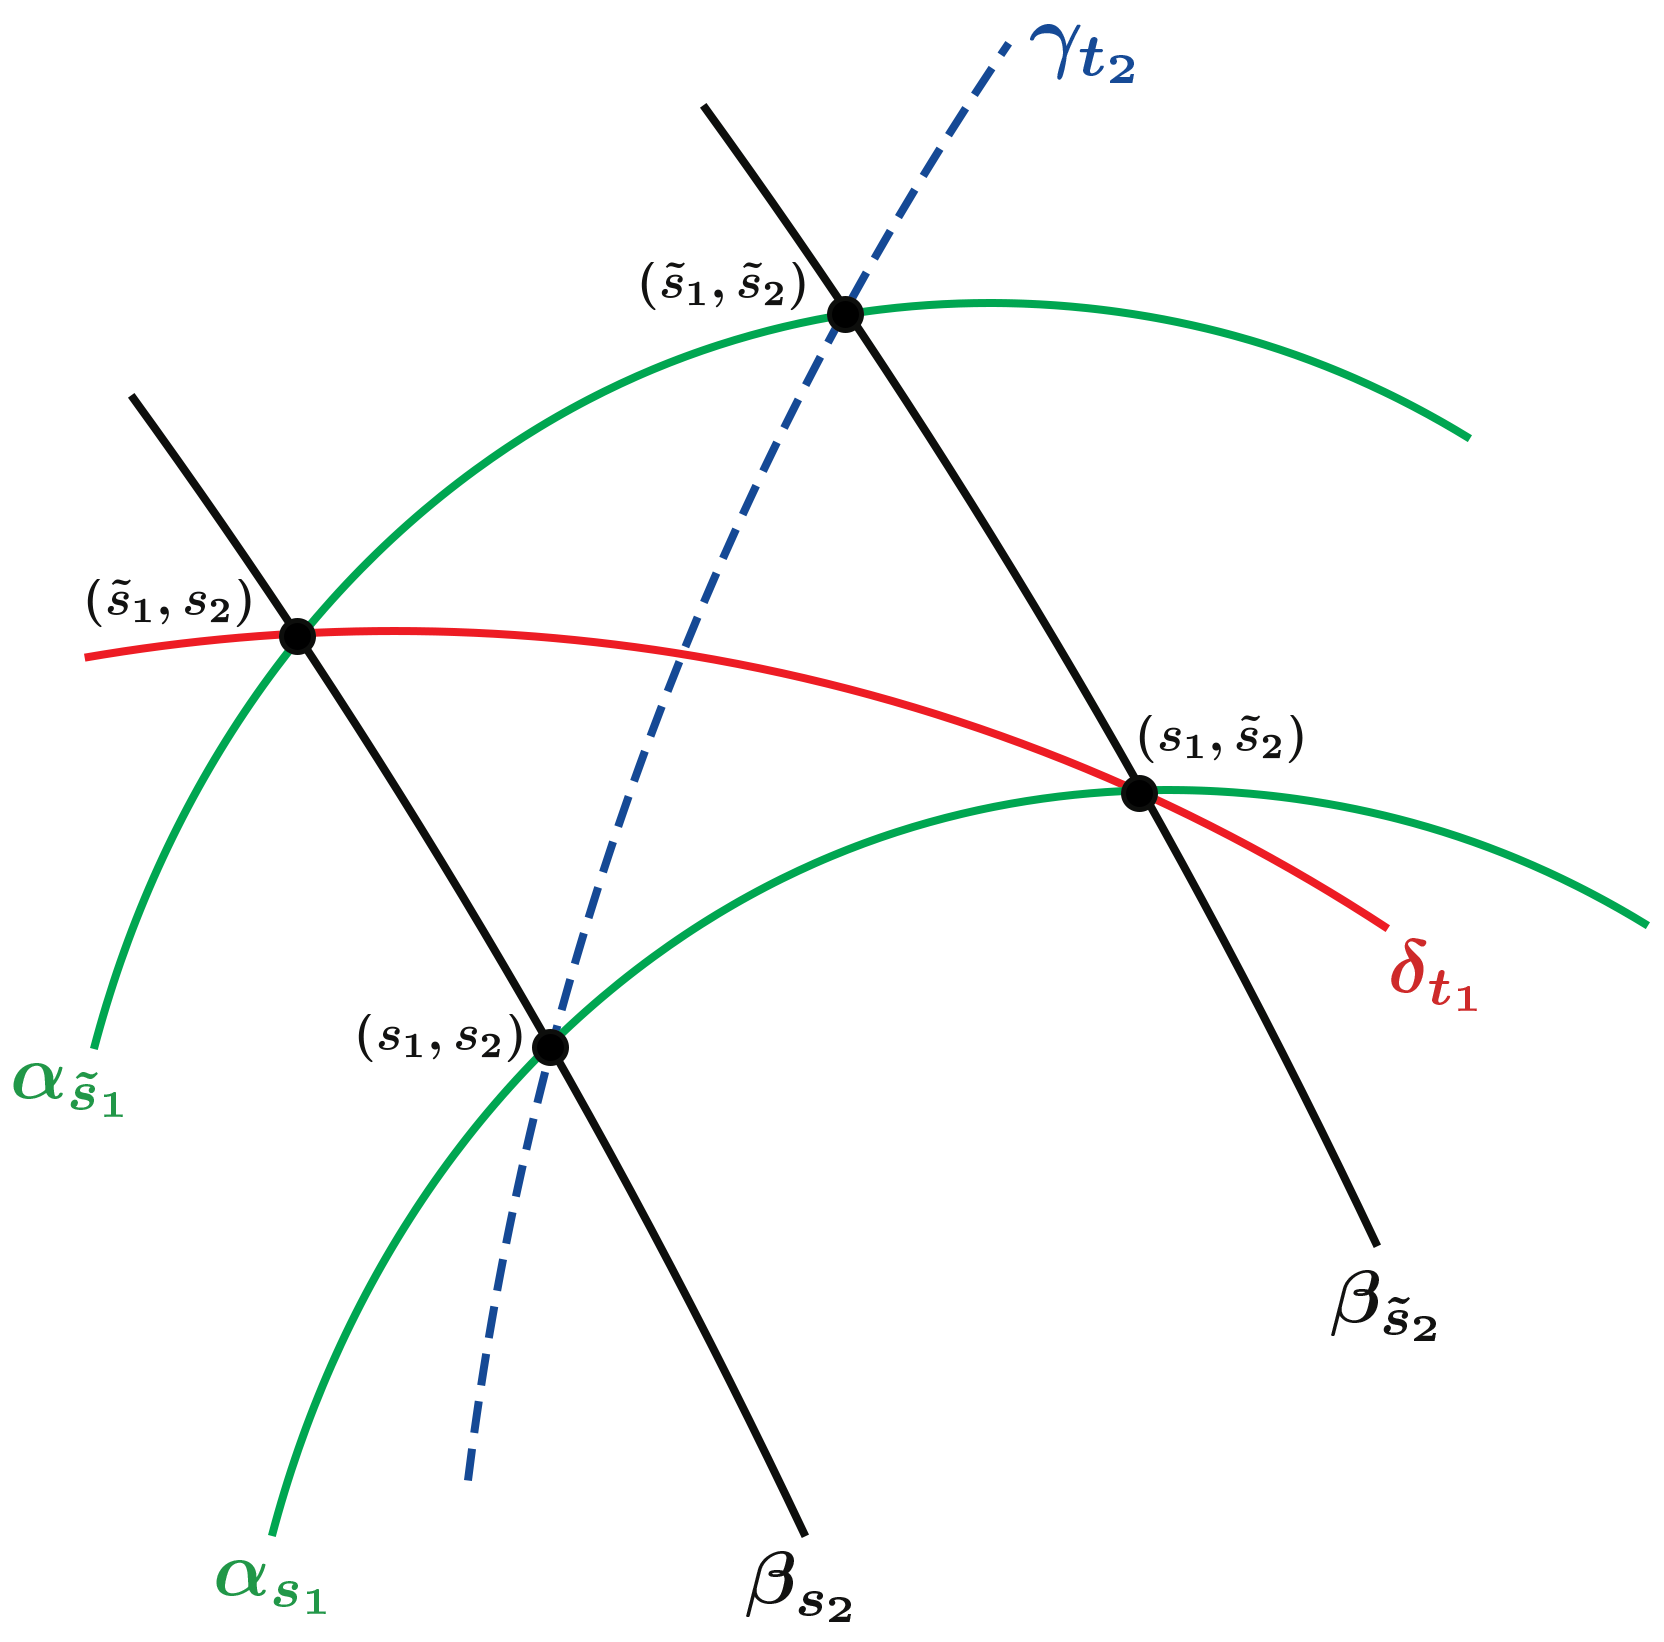
\includegraphics[width=0.5\textwidth]{diagonally_related_diagram.png}
    \caption{An illustration of the diagonal relation between two nets.}
    \label{fig:diagonally-related-diagram}
\end{figure}

\begin{theorem}[]
\label{thm:symmetric-definition-diagonal-nets}
Let $\mathcal{N}_1$ and $\mathcal{N}_2$ be two nets on a surface $\Sigma$. Then $\mathcal{N}_1$ is diagonally related to
$\mathcal{N}_2$ if and only if $\mathcal{N}_2$ is diagonally related to $\mathcal{N}_1$.
\end{theorem}

\begin{proof}
    The proof
\end{proof}
\pagebreak
%===========================================================
\section{Diagonally related parameterization of hyperboloids}
\begin{theorem}[]
\label{thm:diagonally-related-one-sheeted}
On any one-sheeted hyperboloid, the net of curvature lines and the net of circular sections are diagonally related.
\end{theorem}
\begin{proof}
    Write
\end{proof}

\begin{theorem}[]
\label{thm:diagonally-related-two-sheeted}
On any two-sheeted hyperboloid, the net of curvature lines and the net of circular sections are diagonally related.
\end{theorem}
\begin{proof}
    Write
\end{proof}
\pagebreak
%===========================================================
\section{Isometric deformation of circular cross sections of hyperboloids}
\begin{theorem}
\label{thm:affine-transformation-one-sheeted}
Let $\alpha > \beta > \gamma > 0$ and $\mathcal{H}_{1}$ be the one-sheeted hyperboloid \eqref{eq:two-sheeted-alpha-beta-gamma}. Then, there exists a one-parameter family of affine transformations given by
\[
    \mathbb{R}^3 \to \mathbb{R}^3 \quad \quad (x, y, z) \mapsto (\sigma_{1}x, \sigma_{2}y, \sigma_{3}z)
\]
with $\sigma_{1}, \sigma_{2}, \sigma_{3} > 0$ and
\begin{equation}
    \beta(\alpha + \gamma) \sigma_{2}^2 + \gamma(\alpha - \beta) \sigma_{3}^2 = \alpha (\beta + \gamma)
\end{equation}
that is isometric on the circular sections of $\mathcal{H}_{1}$. Any affine transforms of $\mathcal{H}_1$ under this map are confocal up to scaling.
\end{theorem}
\begin{proof}
    Write
\end{proof}

\begin{theorem}
\label{thm:affine-transformation-two-hyperboloid}
Let $\alpha > \beta > \gamma > 0$ and $\mathcal{H}_{2}$ be the two-sheeted hyperboloid \eqref{eq:two-sheeted-alpha-beta-gamma}. Then, there exists a one-parameter family of affine transformations given by
\[
    \mathbb{R}^3 \to \mathbb{R}^3 \quad \quad (x, y, z) \mapsto (\sigma_{1}x, \sigma_{2}y, \sigma_{3}z)
\]
with $\sigma_{1}, \sigma_{2}, \sigma_{3} > 0$ and
\begin{equation}
    \beta (\alpha + \gamma) \sigma_{2}^2 - \alpha (\beta - \gamma) \sigma_{1}^2 = \gamma (\alpha + \beta)
\end{equation}
that is isometric on the circular sections of $\mathcal{H}_{2}$. Any affine transforms of $\mathcal{H}_1$ under this map are confocal up to scaling.
\end{theorem}
\begin{proof}
    Write
\end{proof}

\begin{theorem}
\label{thm:isometric-deformation-para-one-hyperboloid}
Let $a > b > c > 0$ and $\mathcal{H}_{1}(s_{2})$ be a one-parameter family of one-sheeted hyperboloids given by
\begin{equation}
x^2 + \frac{a - c}{b - c} \frac{y^2}{\sin(s_{2})^2} -  \frac{a - b}{b - c} \frac{z^2}{ \cos(s_{2})^2} = 1.
\end{equation}
Then for each $s_{2} \in \left[ 0, \frac{\pi}{2} \right]$, the two parameterizations
\begin{align*}
    \varphi_{\pm} &: [-s_{1}^{0}, s_{1}^{0}] \times (-\infty, \infty) \to \mathbb{R}^3 \quad \quad (s_{1}, s_{3}) \mapsto (x, y, z) \\[10pt]
    x(s_{1}, s_{2}, s_{3}) &= \pm \sqrt{1 - \frac{b - c}{a - b} \sinh^2(s_{1})} \sqrt{1 + \frac{b - c}{a - c}\sinh^2(s_{3})} \\[10pt]
    y(s_{1}, s_{2}, s_{3}) &= \frac{b - c}{\sqrt{a - b} \sqrt{a - c}} \sinh(s_{1}) \sin(s_{2})\cosh(s_{3}) \\[10pt]
    z(s_{1}, s_{2}, s_{3}) &= \frac{b - c}{\sqrt{a - b} \sqrt{a - c}}  \cosh(s_{1}) \cos(s_{2}) \sinh(s_{3})
\end{align*}
with
\[
    s_{1}^{0} = \sinh^{-1}\left( \sqrt{ \frac{a - b}{b - c} } \right)
\]
are curvature line parameterizations of the two halves $\mathcal{H}_{1}(s_{2}) \cap \{ x \geq 0\}$ and $\mathcal{H}_{1}(s_{2}) \cap \{ x \leq 0\}$ of the one-sheeted hyperboloid, and the curves $s_{1} \pm s_{3} = \text{const.}$ are congruent circles. \newline
This one-parameter family of one-sheeted hyperboloids $\mathcal{H}_{1}(s_{2})$ includes two planar degenerations corresponding to $s_{2} = 0,\left(y = 0 \right)$ and $s_{2} = \pi/2, \left( z = 0 \right)$.
\end{theorem}

\begin{theorem}
\label{thm:isometric-deformation-para-two-hyperboloid}
Let $a > b > c > 0$ and $\mathcal{H}_{2}(s_{1})$ be a one-parameter family of two-sheeted hyperboloids given by
\end{theorem}
%===========================================================
\section{Further related work}
\label{sec:further-related-work}
\subsection{Confocal paraboloids}
\label{subsec:confocal-paraboloids}
\subsection{Discrete confocal quadrics}
\label{subsec:discrete-confocal-quadrics}
\pagebreak
%===========================================================
\appendix
\section{Quadric hypersurfaces}
\label{appendix:quadrics}
\pagebreak
%===========================================================
\section{Curvature line parameterizations}
\label{appendix:curvature-lines}
\pagebreak
%===========================================================


%===========================================================
% Set page style to "tocstyle"
\pagestyle{tocstyle}
\addcontentsline{toc}{section}{Bibliography}
\bibliographystyle{alphaurl}
\bibliography{refs}
%===========================================================


\end{document}
